\documentclass{standalone}
\usepackage{tikz}
\usetikzlibrary{patterns, positioning}
\usepackage[sfdefault]{ClearSans} %% option 'sfdefault' activates Clear Sans as the default text font
\usepackage[T1]{fontenc}

\begin{document}
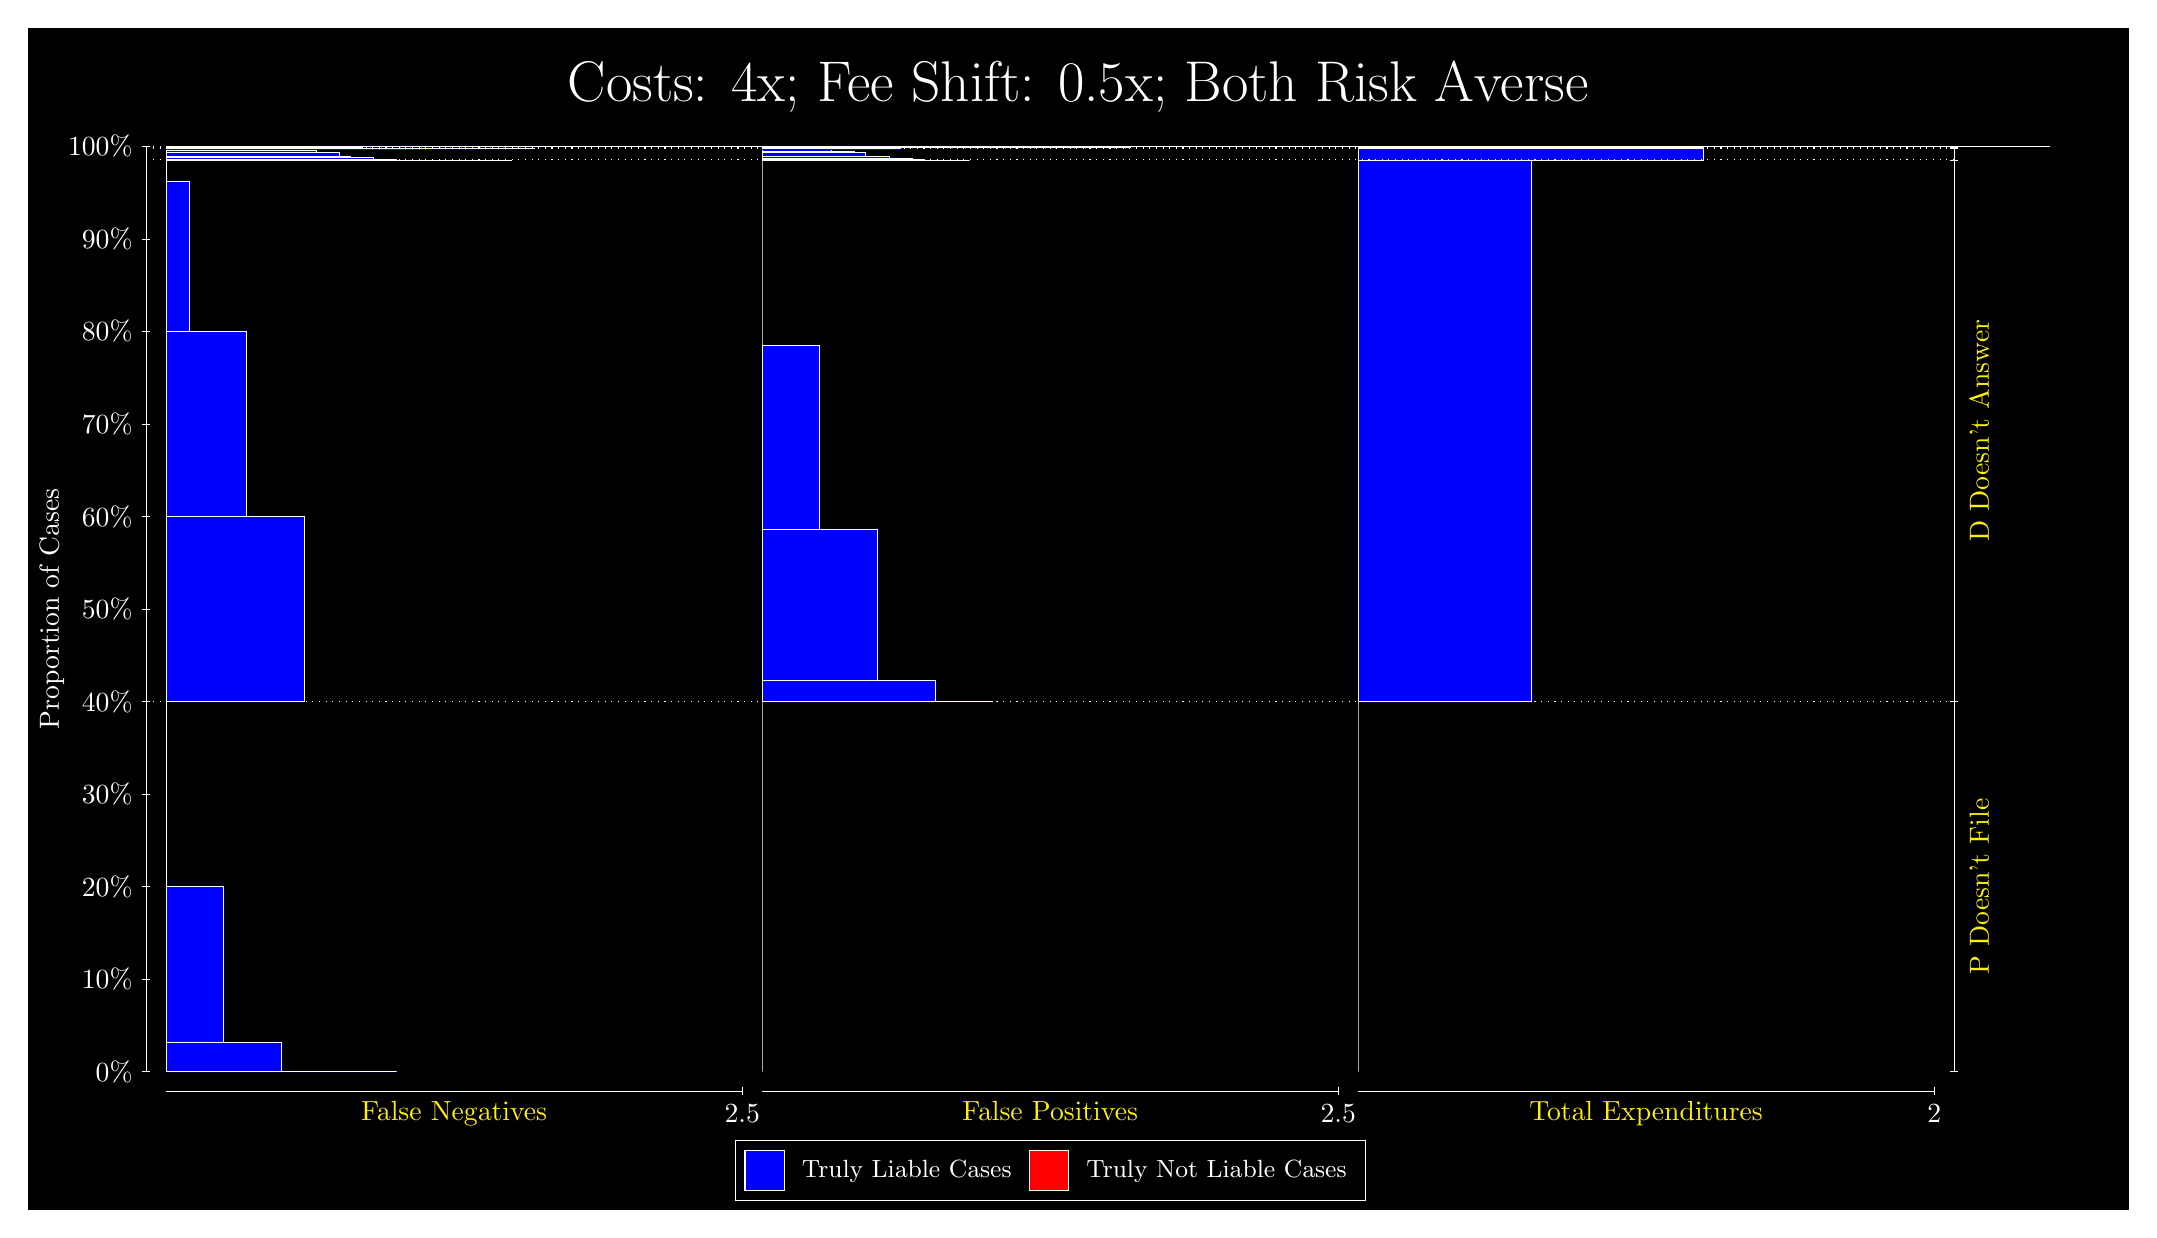
\begin{tikzpicture}
\draw[fill=black] (0,0) rectangle (26.667,15);
\draw[text=white] (0,13.5) rectangle (26.667,15) node[midway] {\huge Costs: 4x; Fee Shift: 0.5x; Both Risk Averse};
\draw[white, very thin] (1.5,1.75) -- (1.5,13.5);
\node[rotate=90, text=white, anchor=center] at (0.3, 7.625) {Proportion of Cases};
\draw[white, very thin] (1.45,1.75) -- (1.55,1.75);
\node[text=white, anchor=east] at (1.45, 1.75) {0\%};
\draw[white, very thin] (1.45,2.925) -- (1.55,2.925);
\node[text=white, anchor=east] at (1.45, 2.925) {10\%};
\draw[white, very thin] (1.45,4.1) -- (1.55,4.1);
\node[text=white, anchor=east] at (1.45, 4.1) {20\%};
\draw[white, very thin] (1.45,5.275) -- (1.55,5.275);
\node[text=white, anchor=east] at (1.45, 5.275) {30\%};
\draw[white, very thin] (1.45,6.45) -- (1.55,6.45);
\node[text=white, anchor=east] at (1.45, 6.45) {40\%};
\draw[white, very thin] (1.45,7.625) -- (1.55,7.625);
\node[text=white, anchor=east] at (1.45, 7.625) {50\%};
\draw[white, very thin] (1.45,8.8) -- (1.55,8.8);
\node[text=white, anchor=east] at (1.45, 8.8) {60\%};
\draw[white, very thin] (1.45,9.975) -- (1.55,9.975);
\node[text=white, anchor=east] at (1.45, 9.975) {70\%};
\draw[white, very thin] (1.45,11.15) -- (1.55,11.15);
\node[text=white, anchor=east] at (1.45, 11.15) {80\%};
\draw[white, very thin] (1.45,12.325) -- (1.55,12.325);
\node[text=white, anchor=east] at (1.45, 12.325) {90\%};
\draw[white, very thin] (1.45,13.5) -- (1.55,13.5);
\node[text=white, anchor=east] at (1.45, 13.5) {100\%};

\draw[white, very thin] (24.457,1.75) -- (24.457,13.5);
\draw[white, very thin] (24.407,1.75) -- (24.507,1.75);
\node[anchor=west] at (24.407, 1.75) {};
\draw[white, very thin] (24.407,6.4489) -- (24.507,6.4489);
\node[anchor=west] at (24.407, 6.4489) {};
\draw[white, very thin] (24.407,13.329) -- (24.507,13.329);
\node[anchor=west] at (24.407, 13.329) {};
\draw[white, very thin] (24.407,13.47) -- (24.507,13.47);
\node[anchor=west] at (24.407, 13.47) {};
\draw[white, very thin] (24.407,13.487) -- (24.507,13.487);
\node[anchor=west] at (24.407, 13.487) {};
\draw[white, very thin] (24.407,13.499) -- (24.507,13.499);
\node[anchor=west] at (24.407, 13.499) {};
\draw[white, very thin] (24.407,13.5) -- (24.507,13.5);
\node[anchor=west] at (24.407, 13.5) {};

\draw[white, very thin, fill=blue] (1.75,1.75) rectangle (4.6775,1.75);
\draw[white, very thin, fill=blue] (1.75,1.75) rectangle (3.9457,1.7532);
\draw[white, very thin, fill=blue] (1.75,1.7532) rectangle (3.2138,2.126);
\draw[white, very thin, fill=blue] (1.75,2.126) rectangle (2.4819,4.1027);
\draw[white, very thin, fill=red] (1.75,4.1027) rectangle (1.75,4.1027);
\draw[white, very thin, fill=blue] (1.75,4.1027) rectangle (1.75,6.4489);
\draw[white, very thin, fill=blue] (1.75,6.4489) rectangle (3.5065,8.7989);
\draw[white, very thin, fill=blue] (1.75,8.7989) rectangle (2.7746,11.145);
\draw[white, very thin, fill=blue] (1.75,11.145) rectangle (2.0428,13.061);
\draw[white, very thin, fill=red] (1.75,13.061) rectangle (1.75,13.061);
\draw[white, very thin, fill=blue] (1.75,13.061) rectangle (1.75,13.329);
\draw[white, very thin, fill=blue] (1.75,13.329) rectangle (6.1413,13.329);
\draw[white, very thin, fill=blue] (1.75,13.329) rectangle (5.8486,13.329);
\draw[white, very thin, fill=blue] (1.75,13.329) rectangle (5.5558,13.329);
\draw[white, very thin, fill=blue] (1.75,13.329) rectangle (5.4094,13.329);
\draw[white, very thin, fill=blue] (1.75,13.329) rectangle (5.1167,13.329);
\draw[white, very thin, fill=blue] (1.75,13.329) rectangle (4.8239,13.329);
\draw[white, very thin, fill=blue] (1.75,13.329) rectangle (4.6775,13.331);
\draw[white, very thin, fill=blue] (1.75,13.331) rectangle (4.3848,13.365);
\draw[white, very thin, fill=blue] (1.75,13.365) rectangle (4.092,13.378);
\draw[white, very thin, fill=blue] (1.75,13.378) rectangle (3.9457,13.421);
\draw[white, very thin, fill=blue] (1.75,13.421) rectangle (3.6529,13.456);
\draw[white, very thin, fill=blue] (1.75,13.456) rectangle (3.3602,13.468);
\draw[white, very thin, fill=blue] (1.75,13.468) rectangle (3.2138,13.47);
\draw[white, very thin, fill=blue] (1.75,13.47) rectangle (2.921,13.47);
\draw[white, very thin, fill=blue] (1.75,13.47) rectangle (2.6283,13.47);
\draw[white, very thin, fill=red] (1.75,13.47) rectangle (1.75,13.47);
\draw[white, very thin, fill=blue] (1.75,13.47) rectangle (6.4341,13.47);
\draw[white, very thin, fill=blue] (1.75,13.47) rectangle (5.7022,13.47);
\draw[white, very thin, fill=blue] (1.75,13.47) rectangle (4.9703,13.471);
\draw[white, very thin, fill=blue] (1.75,13.471) rectangle (4.2384,13.486);
\draw[white, very thin, fill=blue] (1.75,13.486) rectangle (3.5065,13.487);
\draw[white, very thin, fill=red] (1.75,13.487) rectangle (1.75,13.487);
\draw[white, very thin, fill=blue] (1.75,13.487) rectangle (3.5065,13.487);
\draw[white, very thin, fill=blue] (1.75,13.487) rectangle (2.7746,13.488);
\draw[white, very thin, fill=blue] (1.75,13.488) rectangle (2.0428,13.499);
\draw[white, very thin, fill=red] (1.75,13.499) rectangle (1.75,13.499);
\draw[white, very thin, fill=blue] (1.75,13.499) rectangle (1.75,13.499);
\draw[white, very thin, fill=blue] (1.75,13.499) rectangle (9.9471,13.499);
\draw[white, very thin, fill=blue] (1.75,13.499) rectangle (9.2152,13.499);
\draw[white, very thin, fill=blue] (1.75,13.499) rectangle (8.4834,13.499);
\draw[white, very thin, fill=blue] (1.75,13.499) rectangle (7.7515,13.499);
\draw[white, very thin, fill=blue] (1.75,13.499) rectangle (7.0196,13.499);
\draw[white, very thin, fill=blue] (1.75,13.499) rectangle (5.7022,13.499);
\draw[white, very thin, fill=blue] (1.75,13.499) rectangle (4.9703,13.499);
\draw[white, very thin, fill=blue] (1.75,13.499) rectangle (4.2384,13.499);
\draw[white, very thin, fill=blue] (1.75,13.499) rectangle (3.5065,13.5);
\draw[white, very thin, fill=blue] (1.75,13.5) rectangle (2.7746,13.5);
\draw[white, very thin, fill=blue] (1.75,13.5) rectangle (2.0428,13.5);
\draw[white, very thin, fill=red] (1.75,13.5) rectangle (1.75,13.5);
\draw[white, very thin, fill=blue] (1.75,13.5) rectangle (1.75,13.5);
\draw[white, very thin, fill=red] (9.3189,1.75) rectangle (9.3189,1.75);
\draw[white, very thin, fill=blue] (9.3189,1.75) rectangle (9.3189,6.4489);
\draw[white, very thin, fill=red] (9.3189,6.4489) rectangle (12.246,6.4489);
\draw[white, very thin, fill=blue] (9.3189,6.4489) rectangle (12.246,6.4495);
\draw[white, very thin, fill=blue] (9.3189,6.4495) rectangle (11.515,6.7163);
\draw[white, very thin, fill=blue] (9.3189,6.7163) rectangle (10.783,8.6326);
\draw[white, very thin, fill=blue] (9.3189,8.6326) rectangle (10.051,10.979);
\draw[white, very thin, fill=blue] (9.3189,10.979) rectangle (9.3189,13.329);
\draw[white, very thin, fill=red] (9.3189,13.329) rectangle (11.954,13.329);
\draw[white, very thin, fill=blue] (9.3189,13.329) rectangle (11.954,13.329);
\draw[white, very thin, fill=red] (9.3189,13.329) rectangle (11.661,13.329);
\draw[white, very thin, fill=blue] (9.3189,13.329) rectangle (11.661,13.329);
\draw[white, very thin, fill=red] (9.3189,13.329) rectangle (11.368,13.329);
\draw[white, very thin, fill=blue] (9.3189,13.329) rectangle (11.368,13.331);
\draw[white, very thin, fill=blue] (9.3189,13.331) rectangle (11.222,13.344);
\draw[white, very thin, fill=blue] (9.3189,13.344) rectangle (10.929,13.379);
\draw[white, very thin, fill=blue] (9.3189,13.379) rectangle (10.636,13.422);
\draw[white, very thin, fill=blue] (9.3189,13.422) rectangle (10.49,13.434);
\draw[white, very thin, fill=blue] (9.3189,13.434) rectangle (10.197,13.469);
\draw[white, very thin, fill=blue] (9.3189,13.469) rectangle (9.9044,13.47);
\draw[white, very thin, fill=blue] (9.3189,13.47) rectangle (9.758,13.47);
\draw[white, very thin, fill=blue] (9.3189,13.47) rectangle (9.4652,13.47);
\draw[white, very thin, fill=blue] (9.3189,13.47) rectangle (9.3189,13.47);
\draw[white, very thin, fill=red] (9.3189,13.47) rectangle (11.075,13.47);
\draw[white, very thin, fill=blue] (9.3189,13.47) rectangle (11.075,13.471);
\draw[white, very thin, fill=blue] (9.3189,13.471) rectangle (10.344,13.487);
\draw[white, very thin, fill=blue] (9.3189,13.487) rectangle (9.6116,13.487);
\draw[white, very thin, fill=blue] (9.3189,13.487) rectangle (9.3189,13.487);
\draw[white, very thin, fill=red] (9.3189,13.487) rectangle (14.003,13.487);
\draw[white, very thin, fill=blue] (9.3189,13.487) rectangle (14.003,13.487);
\draw[white, very thin, fill=blue] (9.3189,13.487) rectangle (13.271,13.488);
\draw[white, very thin, fill=blue] (9.3189,13.488) rectangle (12.539,13.499);
\draw[white, very thin, fill=blue] (9.3189,13.499) rectangle (11.807,13.499);
\draw[white, very thin, fill=blue] (9.3189,13.499) rectangle (11.075,13.499);
\draw[white, very thin, fill=red] (9.3189,13.499) rectangle (17.516,13.499);
\draw[white, very thin, fill=blue] (9.3189,13.499) rectangle (17.516,13.499);
\draw[white, very thin, fill=red] (9.3189,13.499) rectangle (16.784,13.499);
\draw[white, very thin, fill=blue] (9.3189,13.499) rectangle (16.784,13.499);
\draw[white, very thin, fill=red] (9.3189,13.499) rectangle (16.052,13.499);
\draw[white, very thin, fill=blue] (9.3189,13.499) rectangle (16.052,13.499);
\draw[white, very thin, fill=red] (9.3189,13.499) rectangle (15.32,13.499);
\draw[white, very thin, fill=blue] (9.3189,13.499) rectangle (15.32,13.499);
\draw[white, very thin, fill=blue] (9.3189,13.499) rectangle (14.588,13.5);
\draw[white, very thin, fill=blue] (9.3189,13.5) rectangle (13.857,13.5);
\draw[white, very thin, fill=blue] (9.3189,13.5) rectangle (13.125,13.5);
\draw[white, very thin, fill=blue] (9.3189,13.5) rectangle (12.393,13.5);
\draw[white, very thin, fill=red] (9.3189,13.5) rectangle (11.075,13.5);
\draw[white, very thin, fill=blue] (9.3189,13.5) rectangle (11.075,13.5);
\draw[white, very thin, fill=blue] (9.3189,13.5) rectangle (10.344,13.5);
\draw[white, very thin, fill=blue] (9.3189,13.5) rectangle (9.6116,13.5);
\draw[white, very thin, fill=blue] (9.3189,13.5) rectangle (9.3189,13.5);
\draw[white, very thin, fill=red] (16.888,1.75) rectangle (16.888,1.75);
\draw[white, very thin, fill=blue] (16.888,1.75) rectangle (16.888,6.4489);
\draw[white, very thin, fill=red] (16.888,6.4489) rectangle (19.083,6.4489);
\draw[white, very thin, fill=blue] (16.888,6.4489) rectangle (19.083,13.329);
\draw[white, very thin, fill=red] (16.888,13.329) rectangle (21.279,13.329);
\draw[white, very thin, fill=blue] (16.888,13.329) rectangle (21.279,13.47);
\draw[white, very thin, fill=red] (16.888,13.47) rectangle (21.279,13.47);
\draw[white, very thin, fill=blue] (16.888,13.47) rectangle (21.279,13.487);
\draw[white, very thin, fill=red] (16.888,13.487) rectangle (21.279,13.487);
\draw[white, very thin, fill=blue] (16.888,13.487) rectangle (21.279,13.499);
\draw[white, very thin, fill=red] (16.888,13.499) rectangle (25.67,13.499);
\draw[white, very thin, fill=blue] (16.888,13.499) rectangle (25.67,13.5);
\draw[white, dotted] (1.5,6.4489) -- (24.457,6.4489);
\draw[white, dotted] (1.5,13.329) -- (24.457,13.329);
\draw[white, dotted] (1.5,13.47) -- (24.457,13.47);
\draw[white, dotted] (1.5,13.487) -- (24.457,13.487);
\draw[white, dotted] (1.5,13.499) -- (24.457,13.499);
\draw[white, very thin] (1.75,1.5) -- (9.0689,1.5);
\node[text=yellow, anchor=north] at (5.4094, 1.5) {False Negatives};
\draw[white, very thin] (9.0689,1.45) -- (9.0689,1.55);
\node[text=white, anchor=north] at (9.0689, 1.45) {2.5};

\draw[white, very thin] (9.3189,1.5) -- (16.638,1.5);
\node[text=yellow, anchor=north] at (12.978, 1.5) {False Positives};
\draw[white, very thin] (16.638,1.45) -- (16.638,1.55);
\node[text=white, anchor=north] at (16.638, 1.45) {2.5};

\draw[white, very thin] (16.888,1.5) -- (24.207,1.5);
\node[text=yellow, anchor=north] at (20.547, 1.5) {Total Expenditures};
\draw[white, very thin] (24.207,1.45) -- (24.207,1.55);
\node[text=white, anchor=north] at (24.207, 1.45) {2};

\node[text=yellow, centered, rotate=90] at (24.777, 4.0995) {P Doesn't File};
\node[text=yellow, centered, rotate=90] at (24.777, 9.8889) {D Doesn't Answer};





\draw (12.978300999999998,1.5) node[draw=none] (baseCoordinate) {};
\begin{scope}[align=center]
        \matrix[scale=0.5, draw=white, below=0.5cm of baseCoordinate, nodes={draw}, column sep=0.1cm]{
            \node[rectangle, draw, minimum width=0.5cm, minimum height=0.5cm, fill=blue] {}; &
            \node[draw=none, font=\small, text=white] (B) {Truly Liable Cases}; &
            \node[rectangle, draw, minimum width=0.5cm, minimum height=0.5cm, fill=red] {}; &
            \node[draw=none, font=\small, text=white] (B) {Truly Not Liable Cases}; \\
            };
\end{scope}

\end{tikzpicture}
\end{document}